\paragraph{subtraction\_u32}

U32SubtractionGate is a gate to perform a subtraction on 32-bit limbs: given `x', `y', and `borrow', it returns 
the result $x - y - \text{borrow}$ and, if this underflows, a new `borrow'.

Gate structure is like \figref{fig:subtraction-u32}.

\begin{figure}[!ht]
    \centering
    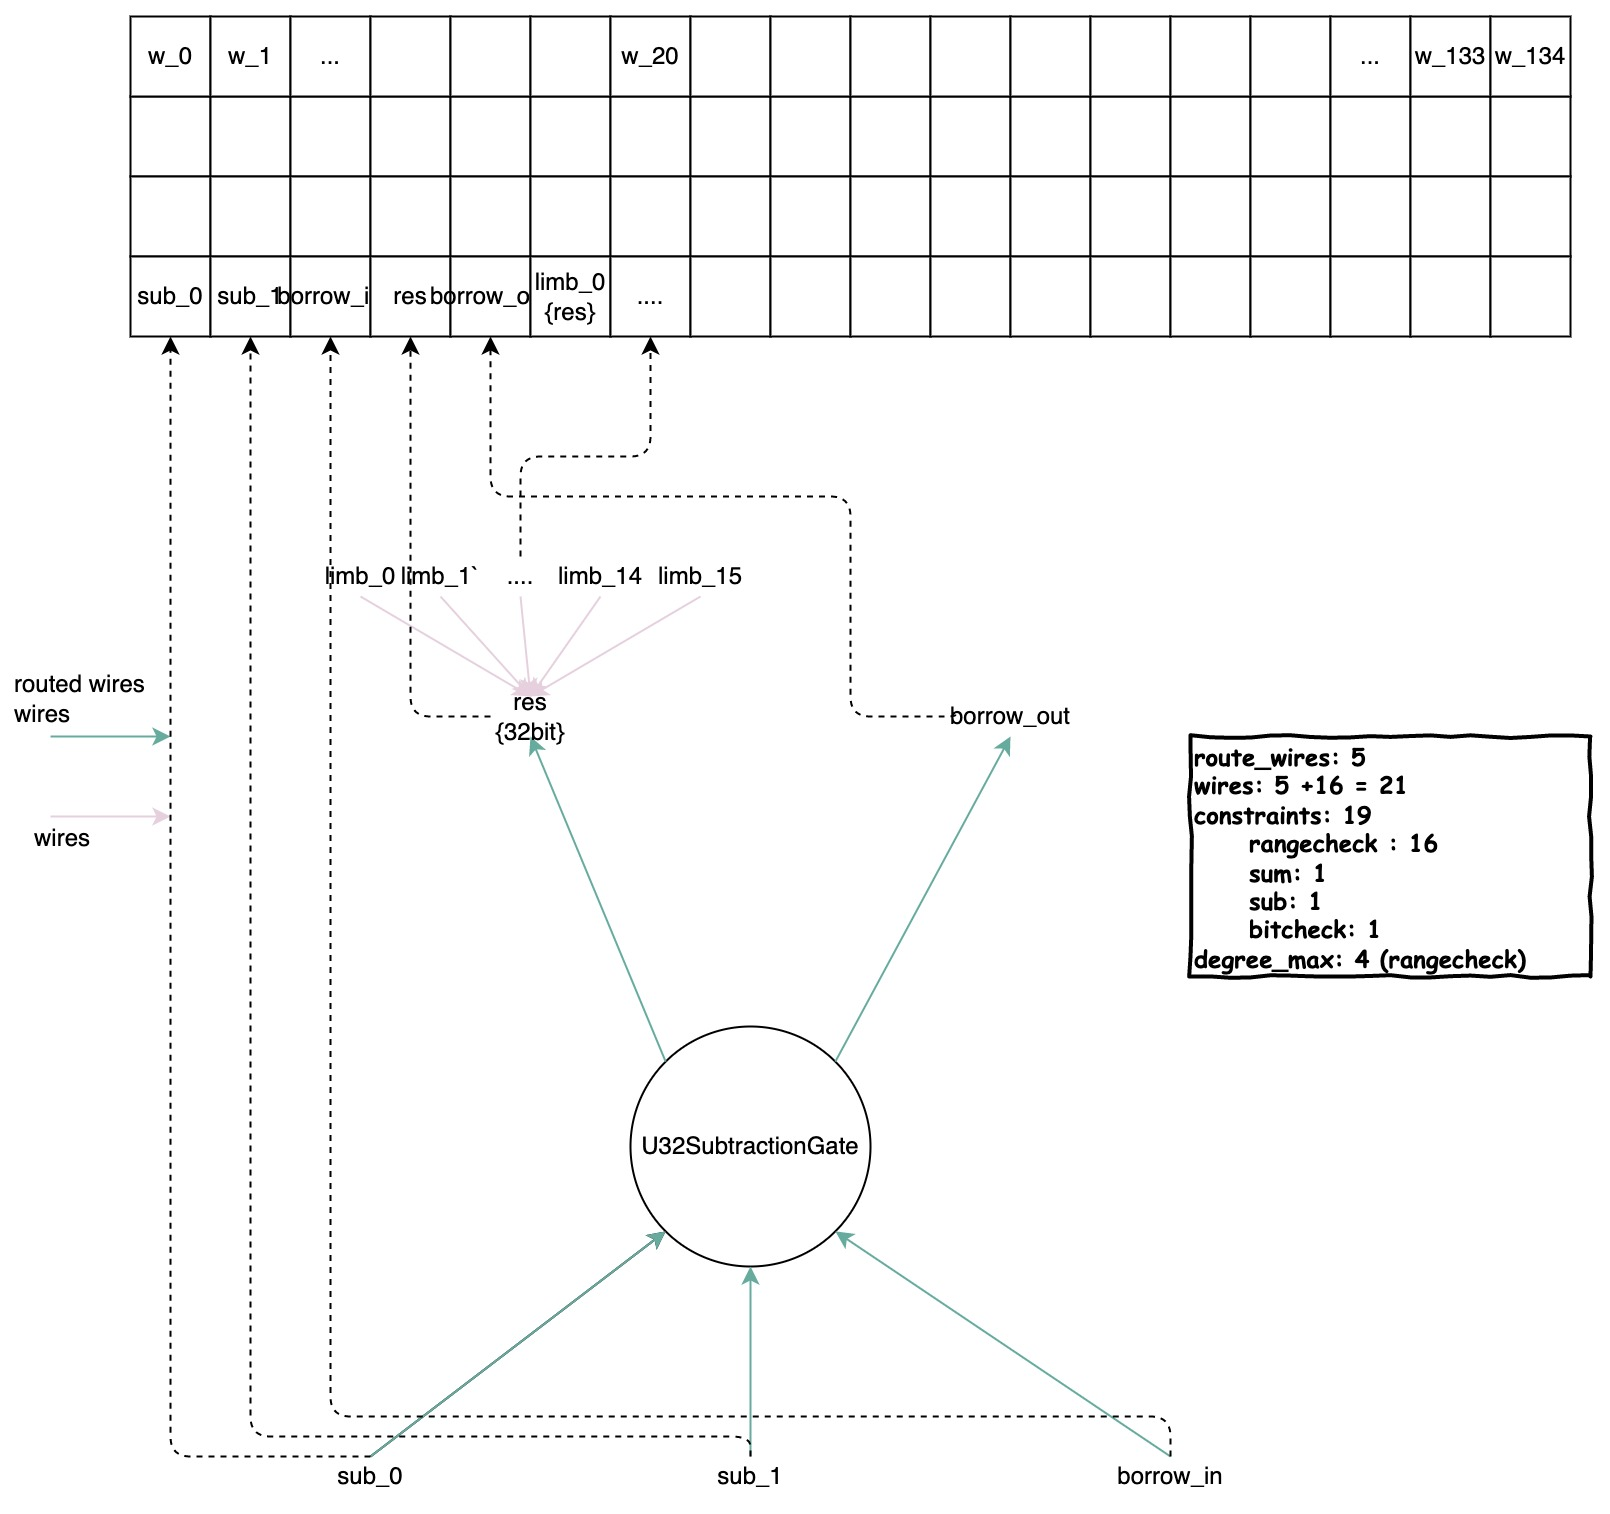
\includegraphics[width=0.6\textwidth]{gates/subtraction_u32.jpeg}
    \caption{U32SubtractionGate}
    \label{fig:subtraction-u32}
\end{figure}

Constraints for each operation:
\begin{itemize}
    \item Constrain the calculation. -- 1 constraint with degree 2.
    \begin{lstlisting}[language=rust]
let result_initial = input_x - input_y - input_borrow;
...
constraints.push(output_result - (result_initial + base * output_borrow));
    \end{lstlisting}
    \item Limbs range check. -- 16 (limbs) constraints with degree 4. (limbs are all 2-bits)
    \item Constrain limbs for res. -- 1 constraint with degree 1.
    \item Constrain borrow\_out to be one bit. -- 1 constraint with degree 1.
\end{itemize}

In summary, there are 19 constraints for each operation. Degree of the gate is 4 which is needed by 4-bits limbs range check.
